% !TEX TS-program = xelatex
% !TEX encoding = UTF-8 Unicode

\providecommand{\home}{../..}
\documentclass[\home/main.tex]{subfiles}

\begin{document}

\graphicspath{{\home/figures}}

\setlaymanexpl{We develop a cloth simulation on GPU and integrate it in the robotics simulator of the Unity game engine to train a robot to fold cloth.}
\chapter{Robotic folding in simulation}\label{ch:simulation}

% https://ieeexplore.ieee.org/stamp/stamp.jsp?tp=&arnumber=9386154
% https://www.osrfoundation.org/wordpress2/wp-content/uploads/2015/04/roscon2014_scpeters.pdf

The previous chapter discussed that simulators are omnipresent in the robotics community.
In this chapter, we zoom in on this observation by exploring the use of simulation for training robotic controllers for deformable object manipulation. First, we define the components that make up a robotics simulator. Then, we compare different simulation technologies and finally discuss results on learning to fold in simulation.

\section{Digital twins}

% Why use simulation: rise of virtual env "digital twin"
Using a digital representation of a robot and the environment in which it operates allows reducing costly time on the real robot. This use-case has given rise to the term \emph{digital twin} meaning that the physical platform has a virtual representation which can be utilized. This digital twin is a cost-effective tool for learning and safe experimentation. These benefits have proven their merit in the robotics field which has led to a plethora of simulator choices available to researchers \autocite{Collins2021}. However, navigating the simulation landscape is difficult and requires pinpointing exact requirements. For researching the use of simulation for learning to fold cloth, we discuss the following requirements in this section:
\begin{itemize}
    \item The simulation tool needs to be able to simulate robots and the associated physics.
    \item In addition to the rigid body simulation, our research requires simulating cloth dynamics.
    \item To bridge the virtual environment to the physical world, the simulation requires functionality to communicate with the physical robot.
    \item Machine learning and reinforcement learning libraries often require a Python interpreter. Hence, the simulation environment should be able to be interfaced with from Python.
\end{itemize}

% What do we need: our use-case 

\section{Robotic simulation}

% What is a robot simulator and how does it differ from physics simulator. Also real integrations: URDF, ROS communication with real robot. 
A robotic simulator encapsulates a physics simulator while exposing other functionalities specific to solving tasks with robots. The physics simulation, also called physics engine, provides realistic modelling and simulation of physical phenomena. This includes handling the construction and articulation of kinematic chains, querying collision detection, providing friction models and optionally has built-in soft body support.
The distinction between physics and robotic simulations helps understanding the simulators landscape as some physics engines have developed into robotics engines and can be found as physics backend in other robotic simulators.
In \cref{sec:lit_simulation}, we discussed two categories of physics engines: real-time and offline. For robotic learning purposes, we prioritize simulation speed above accuracy so we only consider real-time physic engines. There is a wide variety of real-time physics simulators available such as Bullet \autocite{Bullet}, PhysX \autocite{PhysX}, Havok \autocite{Havok}, ODE \autocite{ODE} and MuJoCo \autocite{Mujoco}.
% Problem with many physics engines: cartesian instead of joint representation
With the exception of MuJoCo, these physics engines are primarily developed for gaming purposes that require real-time simulation. However, in gaming and modelling applications, most bodies have few or even none joints or constraints. Consequently, many physics engines model physical bodies with a Cartesian representation in which each rigid body has 6 degrees of freedom. The joints of a body then becomes constraints imposed on the $6N$-dimensional space. This is in contrast to robots that are multi-body systems of $N$ constrainted links that makes the system dimensionality much closer to $N$ instead of $6N$. Hence, we have a strong preference for robotic simulators that have underlying physic engines using generalized joint coordinates that provide better stability, speed and accuracy. The difference between generalized coordinates versus Cartesian coordinates representation is illustrated in \cref{fig:generalized_vs_cartesian_coordinates}. This example demonstrates that an inverted double pendulum can be represented as a 12 degrees of freedom system with 10 constraints or as a 2 degrees of freedom system without constraints.

\begin{figure}
    \centering
    \subfile{figures/fig_double_pendulum.tex}
    \caption[Comparison between generalized and Cartesian coordinates for representing multibody kinematic chains.]{\textbf{Comparison between generalized and Cartesian coordinates for representing multibody kinematic chains.} An inverted double pendulum can be represented as two links each having 6 degrees of freedom: 3 possible translations and 3 possible rotations. The rotations $\phi_i, \theta_i, \psi_i$ refer to roll, pitch, yaw respectively. In this \textcolor{ColorAccent1Strong}{Cartesian representation}, indicated in \textcolor{ColorAccent1Strong}{red}, all translations and 2 rotations are constrained per link. The \textcolor{ColorAccent2Strong}{joint coordinate representation}, indicated in \textcolor{ColorAccent2Strong}{yellow}, on the other hand does not have to impose any constraints because it represents the system with 2 degrees of freedom $\alpha_1$ and $\alpha_2$.}
    \label{fig:generalized_vs_cartesian_coordinates}
\end{figure}

% Other robotic simulator functionality
On top of integrating a physics simulation, the robotic simulator exposes functionality specific to the robotics domain.
% URDF
One of these features is importing predescriped robot models that are often expressed in the Unified Robot Description Format\footnote{\url{http://wiki.ros.org/urdf}}.
% Actuators, control modes
The simulator must provide actuator models for position control, velocity control, and torque control in order to control the physical arms.
% IK, FK
Forward kinematics and inverse kinematics are needed for path planning functionality.
% Sensors
Typically, robots for manipulation tasks are equipped with various sensors such as RGB-D cameras, torque and force sensors which need to be supported by the simulator as well.
% Rendering
Similarly to RGB-D cameras, the simulator benefits from having a rendering pipeline for visualization and debugging purposes. This rendering pipeline can be used as RGB-D camera and is preferably able to execute headless for server-side rendering.
% ROS
In order for the digital twin to communicate with its physical counterpart, it needs messaging channels to the real platform. The communication is often provided through ROS\footnote{\url{https://www.ros.org}}; a middleware software suit providing hardware abstraction through message-passing nodes.
% Python bindings
Finally, we want the robotic simulator to interface with Python interpreters given that the large bulk of machine learning research and libraries are written in Python. Python bindings also allows us to circumvent the explicit need of a robotics simulator with ROS integration as the robot used in this research has direct communication channels in Python.

\subsection{Qualitative comparison of popular robot simulation technologies}
% Short comparison of robot simulation technologies
Performing an in-depth, exhaustive comparison between popular robotics simulators for manipulation tasks is non-trivial. A thorough comparison would require setting up multiple scenarios, relevant metrics and experience with all the considered simulation technologies. For example, it is unclear whether we should compare accuracy, scalability, stability or speed. Furthermore, it is hard to concretely quantify such metrics. For example, accuracy is difficult to quantify in the absence of analytical solutions.
Another metric we could consider is performance in the context of the robotic manipulation tasks. However, the taks performance also depends heavily on the used controller. \textcite{Giovanni2011} for example, found that the simulation engine does not matter when using robust controllers for generating gaits.
Given that all robotic simulators at the time did not provide adequate cloth simulation support, we instead performed a qualitative tradeoff, consulted the documentation, forums and the limited amount of literature available at the time comparing the simulators \autocite{staranowicz2011survey,Erez2015}. We compare the following robotic simulators next: PyBullet, MuJoCo, Gazebo and Unity. Other notable simulators like Taichi \autocite{hu2019taichi}, Isaac\footnote{https://developer.nvidia.com/isaac-sdk} and ThreeDWorld \autocite{gan2021threedworld} are excluded from the current comparison due to not being available or just being released at time of implementing our simulation. A summary of the simulators we considered can be found in \cref{table:comparison_robotic_simulators}.

PyBullet is a robotics framework written in the Python programming language on top of the Bullet physics engine. It provides robot functionality with Python bindings. PyBullet has a focus on machine learning in robotics. At time of executing this research, PyBullet was recently introduced and a one-man effort making the implementation immature. Many features needed yet to be implemented or were not exposed to the Python API. In addition, Bullet recently switched from Cartesian to joint coordinates representation which was not thoroughly debugged. Compared to main-stream game engines, the rendering capabilities of PyBullet are subpar. Finally, PyBullet provides an experimental soft body implementation which we, among other authors \autocite{Matas2018, seita2021learning}, found unuseable. The soft body physics caused cloth to tunnel or explode on grasping attempts and only wireframe rendering was possible at the time. PyBullet has been used for learning to fold cloth \autocite{Matas2018}, learning via virtual reality demonstrations \autocite{mahjourian2019hierarchical} and learning quadruped locomotion with Sim2Real transfer \autocite{tan2018simtoreal}.

Mujoco\textregistered~is a general purpose physics engine developed specifically for robotics research. MuJoCo is generally known for its stable and efficient multibody system dynamics \autocite{Erez2015} and has been used for learning robotic manipulation \autocite{rajeswaran2017learning}, dexterous manipulation \autocite{openai2019solving} and locomotion \autocite{heess2017emergence}. Most of our required features are supported by MuJoCo with the notable exception of inverse kinematics and path planning. At time of executing our research, MuJoCo required a paid license which made it unfit for our purposes to be able to run simulations on remote servers\footnote{MuJoCo was made freely available in October 2021.}. MuJoCo provides volumetric soft body simulation of which the generalization towards planar soft bodies is unclear.

Gazebo is an open-source robotics simulation environment supported by ROS. It exposes multiple physics engines, most notably Bullet and ODE by default. The Bullet physics engine suffers from the shortcomings we mentioned while ODE only offers Cartesian multibody representation, making it slow and potentially unstable for robotics. Gazebo is strongly integrated with the ROS ecosystem, making it very feature-complete for transfer to real robots. None of the physics engines underpinning Gazebo offer decent cloth simulation. Gazebo is widely used in the robotics community, for example autonomous navigation \autocite{Imanberdiyev2016} and visual servoing \autocite{Shi2018}.

Unity\textregistered~is a game engine providing a software development environment and tools for game development. With the Unity ML-Agents toolkit\footnote{\url{https://github.com/Unity-Technologies/ml-agents}}and Unity Robotics Hub\footnote{\url{https://github.com/Unity-Technologies/Unity-Robotics-Hub}}, Unity is laying down a strong footing in the robotics machine learning community. The Unity Robotics Hub enables pulling in functionality from the ROS ecosystem while the Unity ML-Agents toolkit provides a Python API to the underlying simulation environment. Additionally, Unity has integrated the reduced articulation functionality from the PhysX physics engine\footnote{\url{https://gameworksdocs.nvidia.com/PhysX/4.0/documentation/PhysXGuide/Manual/Articulations.html\#reduced-coordinate-articulations}} making multibody simulation like robots physically more accurate with minimal joint errors. The rendering capabilities of Unity are of considerably higher fidelity compared to the previously discussed simulators. The high fidelity is due to the photorealistic rendering capabilities. Unity is being used by AAA game development studios and popular among solo game developers due to the rapid software prototyping tools it provides. Unity has been used for robotic manipulation of soft tissues \autocite{Tagliabue2020} and as backend rendering engine for learning dexterous manipulation \autocite{openai2019solving}.


\begin{table}[htb]
    % \rowcolors{2}{gray!25}{white}

    \begin{threeparttable}

        \centering
        \caption{Qualitative comparison of the robotic simulation technologies considered for learning to fold clothing.}
        \begin{tabular}[t]{@{} l c c c c @{}}
            \toprule
            Requirement             & PyBullet       & MuJoCo                  & Gazebo         & Unity           \\
            \midrule
            Stable physics          & \checkmark     & \checkmark              & \checkmark     & \checkmark      \\
            URDF support            & \checkmark     & \checkmark              & \checkmark     & \checkmark      \\
            Minimal coordinates     & $\pm$\tnote{*} & \checkmark              & $\pm$\tnote{*} & \checkmark      \\
            Python bindings         & \checkmark     & $\pm$\tnote{$\dagger$}  & \checkmark     & \checkmark      \\
            High-fidelity rendering & ---            & ---                     & ---            & \checkmark      \\
            Soft body support       & $\pm$\tnote{*} & $\pm$\tnote{$\ddagger$} & $\pm$\tnote{*} & $\pm$\tnote{*}  \\
            Inverse kinematics      & \checkmark     & $\pm$\tnote{\S}         & \checkmark     & $\pm$\tnote{\S} \\

            \bottomrule
        \end{tabular}
        \begin{tablenotes}\footnotesize
            \item[*] Supported but unmature
            \item[$\dagger$] Via community initiatives
            \item[$\ddagger$] Mature but limited features
            \item[\S] Indirectly, via ROS
        \end{tablenotes}

        \label{table:comparison_robotic_simulators}
    \end{threeparttable}

\end{table}

% why do we go for Unity
Ultimately, we decide to use Unity as robotics research tool. This decision is rationalized by Unity covering most of our required features as shown in \cref{table:comparison_robotic_simulators}. Notably their recent addition of supporting a physics solver for minimal joint coordinate multibodies with the high definition render pipeline sets Unity apart from other simulation technologies. Unity demonstrates to be incumbent player in robotics by dedicating software teams to their ML and robotics department.
Compared to dedicated robotics simulators, Unity produces much higher visual fidelity due to photorealistic rendering. For example, we compare the visuals of a simulated Baxter robot in PyBullet and Unity in \cref{fig:baxter_unity_vs_pybullet}.
In addition, the Unity IDE is a professional and productive working environment. The community is known to be supportive and provides tools for other developers to use. This allows rapid prototyping of new features and experiments. Rapid prototyping together with the above discussed functionality makes Unity a suitable candidate for PhD researchers that are not backed by a large development team.

\begin{figure}[htpb]{}
    \centering
    \begin{subfigure}[b]{0.80\textwidth}
        \centering
        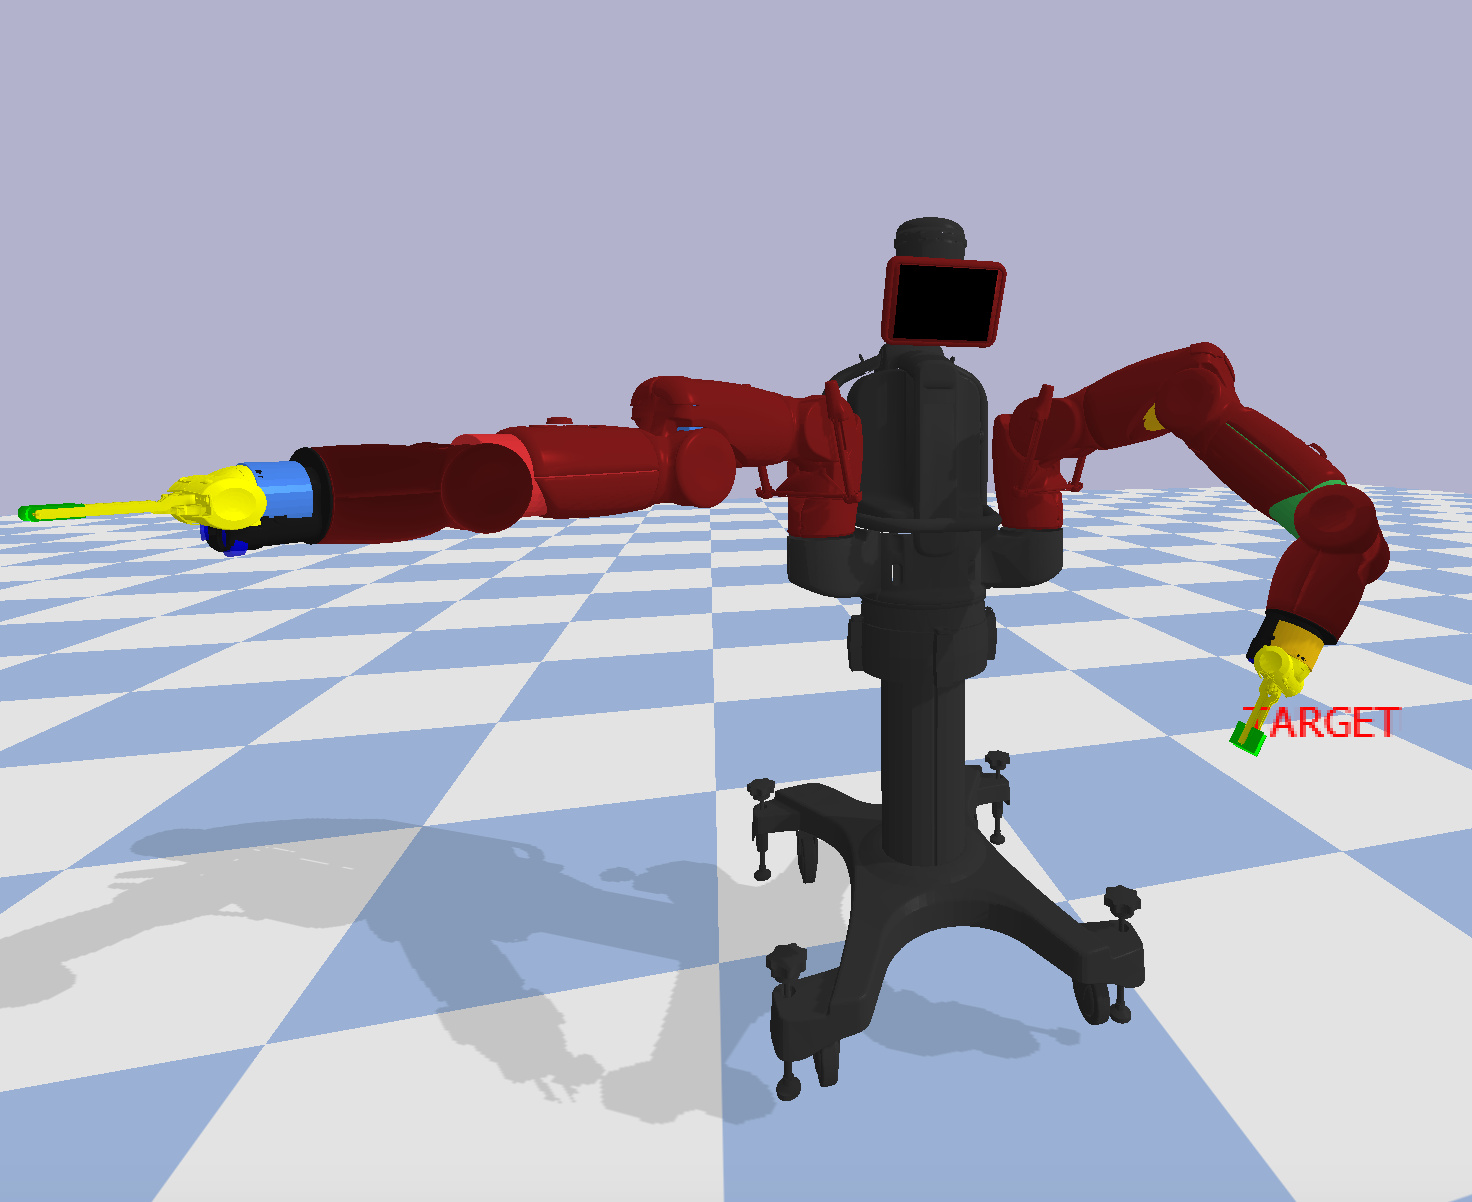
\includegraphics[width=\textwidth]{\home/chapters/04-simulation/figures/baxter_pybullet.jpg}
        \caption{Baxter robot visualization in PyBullet}
        \label{fig:baxter_pybullet}
    \end{subfigure}

    \begin{subfigure}[b]{0.80\textwidth}
        \centering
        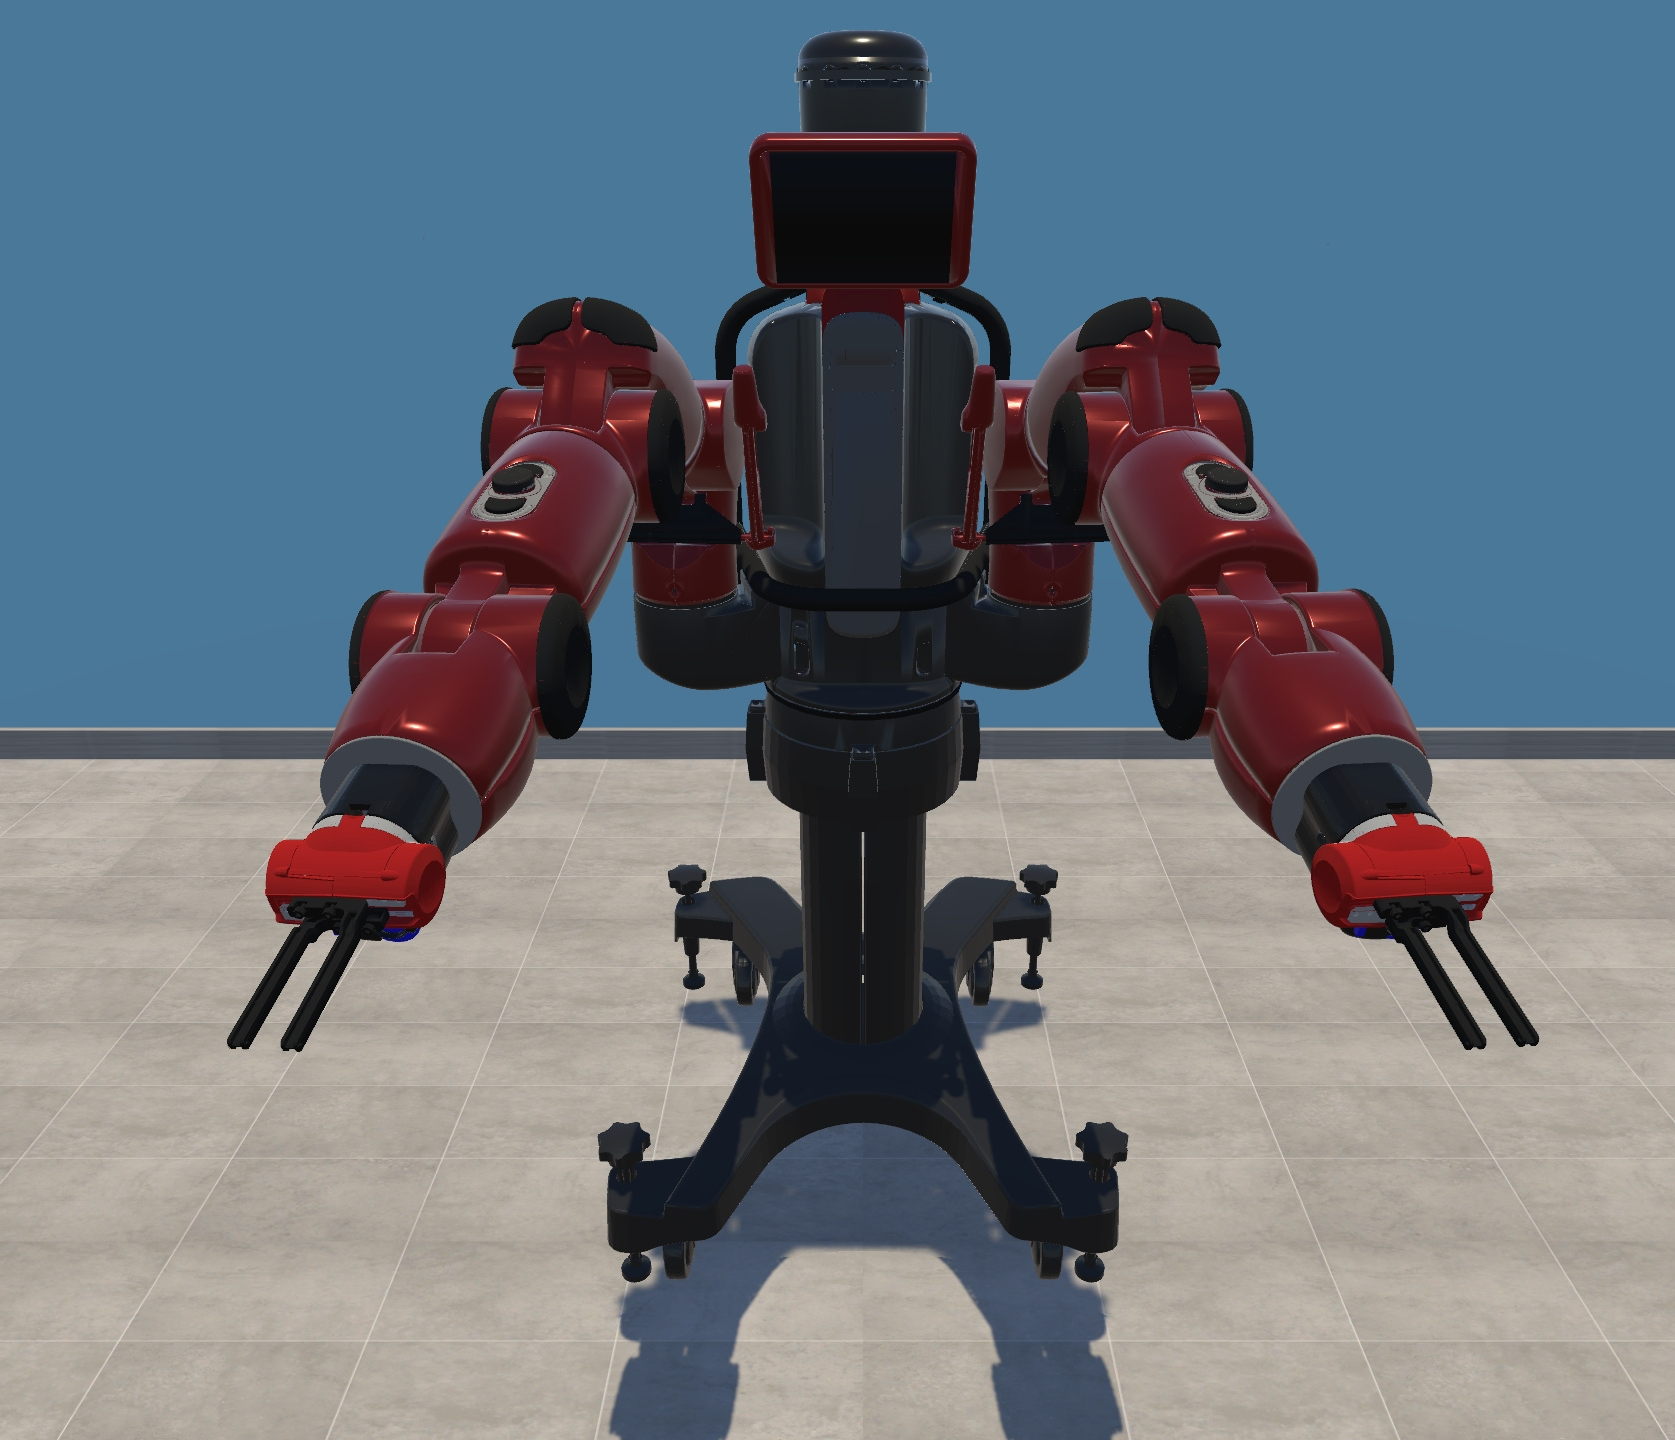
\includegraphics[width=\textwidth]{\home/chapters/04-simulation/figures/baxter_unity.jpg}
        \caption{Baxter robot visualization in Unity}
        \label{fig:baxter_unity}
    \end{subfigure}

    \caption[]{Simulated Baxter: PyBullet vs Unity. The difference in rendering capabilities can be seen in, for example, Unity being able to sample texture images while Bullet uses solid colours. Unity also allows defining the material's roughness; in Unity there is a black, plastic casing around the elbow leading to a complete diffuse light reflection. In contrast, there is a visible specular reflection on elbow joint of Baxter in Bullet. }
    \label{fig:baxter_unity_vs_pybullet}
\end{figure}

% TODO outscope: een tabel maken van aantal papers in de tijd dat welke simulator gebruikt. Om te zien hoe het verschuift. 

\section{Cloth simulation using particle systems}

%Zie ook "Robotic manipulation and sensing of deformable objects in domestic and industrial applications: a survey" p4 voor overzicht om te introduceren maar focus op particle based methods.
%  zie ook Dexterous Robotic Manipulation of Deformable Objects with Multi-Sensory Feedback - a Review van khalil
% background sectie 3 van SoftGym": https://arxiv.org/pdf/2011.07215.pdf
%  Voor de specifieke methode, zie ook p47 van Seita zijn boek 
%  Zie ook Muller notes about deformable object manipulation p11
% diene nederlander zijn cloth sim book
%  diene dude zijn phd over particle system voor tissue simulatie dat ook een blogpost heeft 
% SEL lessen en resultaten group 1


% Cloth simulator: naar wat zijn we opzoek 
Choosing a cloth simulation method requires trading off the geometrical resolution, computational speed, robustness and realism.
The \emph{geometrical} complexity needs to be at a resolution that can accurately represent small deformations and wrinkles that typically appear in clothing items.
The \emph{speed} of the simulation is important for generating massive datasets, which is required when data-hungry learning algorithms are used such as deep neural networks. The computational speed depends on the chosen simulation algorithm, temporal and geometrical resolution.
With \emph{robustness}, we cover requirements such as consistency when repeating the same cloth manipulations and stability when large forces are exerted. For example, game engines apply damping in order to avoid implosion of the forces and corresponding displacements.
Finally, \emph{realism} refers to the realism of the physical behaviour and visual quality. In this regard, we distinguish visual plausibility versus physical plausibility. The former refers to the rendering quality while the latter indicates how realistic the simulated behaviour is. Achieving realistic visualization is possible with modern rendering technologies such as physically based rendering methods that use the principles of physics to model the interaction of light and materials. Contrarily, modelling and tuning physical parameters of a simulation to achieve physical behaviour that follows physics in the real world completely, is difficult. This problem is enlarged in the case of high degree of freedom objects such as clothing articles. Hence, in this regard we prioritize visual fidelity above physical fidelity. Moreover, when using a simulation method, one can tune the degree of realism and geometrical resolution in order to achieve quicker simulation times. In heart surgery simulators for example, it is known that the simulated deformations of tissues do not need to be physically accurate. Instead, the deformations should be consistent and \emph{look} physically realistic \autocite{BroNielsen1998} in order to facilitate the suspension of disbelief.

% Cloth sim 
Modelling consistent and seemingly realistic deformations is the primary challenge for cloth simulation. For example, if we consider cloth to be constituted of $n$ elementary particles, then computation of the forces on a particle requires incorporating pairwise interactions from all other particles leading to a $\mathcal{O}(n^2)$ computation. This computation is challenging to do in real-time given that cloth often uses many vertices. For example, simulating the dress shown in \cref{fig:dress_blender_vertices}, requires calculating forces for the 17244 vertices leading to a computation of $\mathcal{O}(n^2)$ with $n=17244$.
\begin{figure}
    \centering
    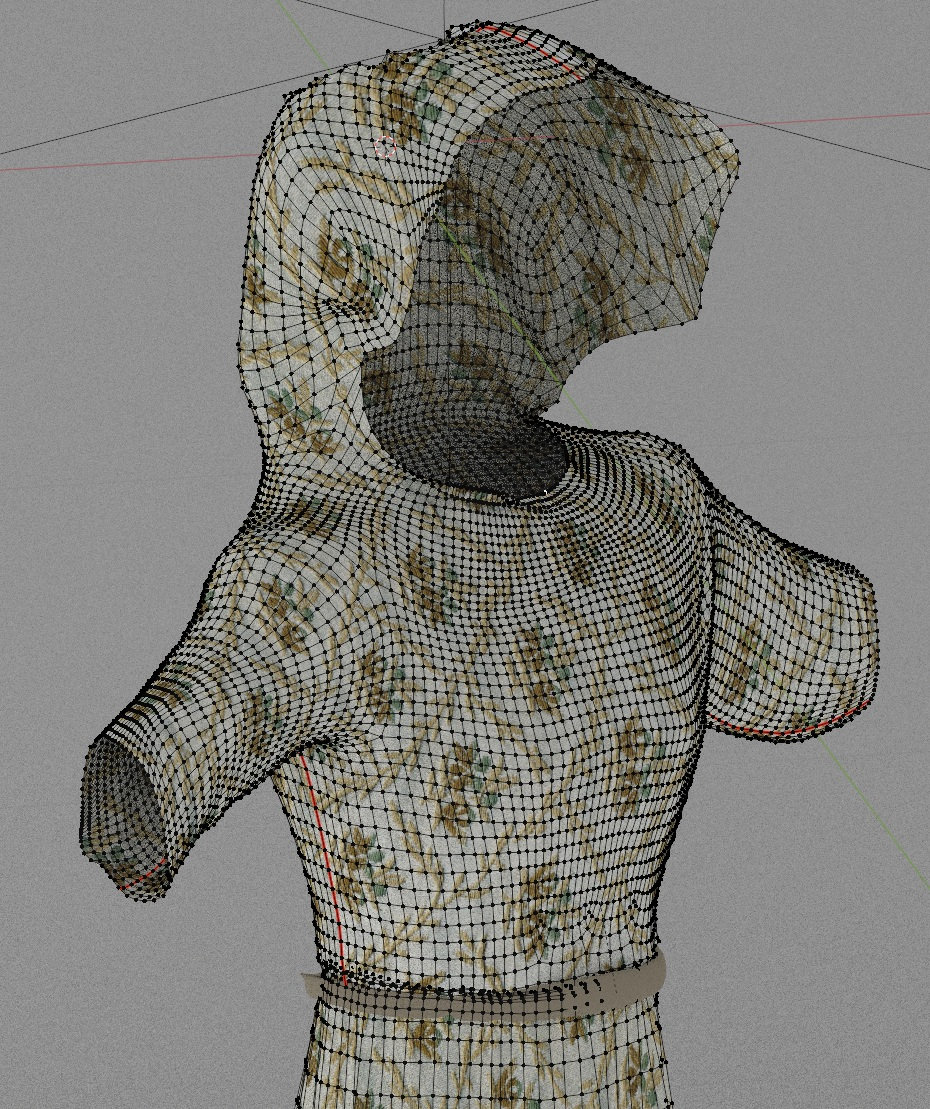
\includegraphics[width=\textwidth]{\home/chapters/04-simulation/figures/dress_blender_vertices.jpg}
    \caption[Example of a 3D modelled dress]{Example of a close-up of 3D modelled dress. The vertices and edges are displayed on top of the mesh. The cloth model and textures were designed by user \textit{mnphmnmn} on turbosquid: \url{https://www.turbosquid.com/Search/Artists/mnphmnmn}.}
    \label{fig:dress_blender_vertices}
\end{figure}

\subsection{Representing cloth with particle systems} \label{subsec:sim_particle_system}

\glsreset{FEM} % because long ago 
In \cref{subsec:lit_cloth_sim} we discussed two popular approaches for soft body simulations: particle systems and \gls{FEM}. To recapitulate; \gls{FEM} is a method to solve continuous equations that govern the behaviour of soft body dynamics by discretizing and linearising the geometry and material properties. The main advantage of \gls{FEM} is physical realism: we calculate approximate solutions to the actual equations governing deformations based on elasticity theory. However, the main problem with \gls{FEM} is simulation speed: each simulation step requires solving a system of equations which is a computationally expensive operation. On the contrary, particle systems combine basic physics and mathematical constraints in order to control the dynamic behaviour of objects. The formulation of particle systems additionally allows to easily exploit dedicated hardware like \glspl{GPU}. For these reasons, we employ a particle-based approach to cloth simulation in this research. We describe particle systems for simulating cloth next.

The computer graphics community has taken a different approach for modelling natural phenomena such as fire, water, foliage, smoke and deformable objects compared to standard computer image synthesis techniques for rigid objects. This is due to the continuously changing, irregular shapes and positions of the elements that make up these phenomena. A well-established method to model such systems is representing each modular atom of the system by a point mass, labelled particle, whose position and velocity are governed by physical laws. This procedural method falls under the category of particle systems. When organizing particles in a fixed topology and connecting neighbouring particles with springs that govern the shape deformation, a spring-mass system is formed.

\begin{figure}[htb]
    \centering
    \subfile{figures/fig_mesh_particles.tex}
    \caption[Mesh of connected particles]{A mesh of connected particles. A particle $p_{i,j}$ is located in row $i$ and column $j$ of the mesh. In this example, each particle is connected only to its first-order neighbourhood.}
    \label{fig:mesh_particles}
\end{figure}

A cloth $\cloth$ is constructed by bundling a collection of connected particles $i \in \cloth$. An example mesh is demonstrated in \cref{fig:mesh_particles}. Each particle contains mass and inertia but does not take up volume. A particle $i$ is defined by a 3D position $\vec{x}_i \in \mathbb{R}^3$ and velocity $\vec{v}_i \in \mathbb{R}^3$. We can organize all positions and velocities of the cloth $\cloth$ with $N$ particles in a vector data structure:
\begin{equation}
    \vec{x}=\left[\begin{array}{c}
            x^{(0)}_{x}   \\
            x^{(0)}_{y}   \\
            x^{(0)}_{z}   \\
            \vdots        \\
            x^{(N-1)}_{x} \\
            x^{(N-1)}_{y} \\
            x^{(N-1)}_{z}
        \end{array}
        \right], \quad \vec{v}=\left[\begin{array}{c}
            v^{(0)}_{x}   \\
            v^{(0)}_{y}   \\
            v^{(0)}_{z}   \\
            \vdots        \\
            v^{(N-1)}_{x} \\
            v^{(N-1)}_{y} \\
            v^{(N-1)}_{z}
        \end{array}\right].
\end{equation}
The position $\vec{x}$ and velocity vector $\vec{v}$ make up the state of the particle system or cloth $\cloth$. The individual positions and velocities are indexed by $v^{(i)}_{x}$ in which superscript $(i)$ indicates particle $i$ and subscript $x$ refers to the $x$-component of the position and velocity vector. The positions $\vec{x}$ and velocities $\vec{v}$ will change over time based on internal spring forces in the cloth and external forces like gravity and interaction with the robot and environment. These forces are obey Newton's second law of motion:
\begin{equation}\label{eq:newton_second_law}
    \vec{f} = m\vec{a},
\end{equation}
where $\vec{f}$ is force, $m$ the mass and $\vec{a}$ acceleration; the first derivative of velocity $\vec{v}$ or the second derivative of position $\vec{x}$.

A spring connects two particles. The types of springs we employ will determine the topology and physics behaviour of the cloth. We elaborate in \cref{subsec:sim_topology_cloth} the type of springs we use for achieving cloth-like behaviour. The springs follow Hook's law: the force exhibited by the spring on the connecting particles is linear in the displacement from the resting distance of the spring. Concretely, the force $\vec{s}_{ij}$ exhibited by the spring connecting particles $i$ and $j$ is given by:
\begin{equation}\label{eq:hook_spring}
    \vec{s}_{ij}=k_{i j}\left(l_{i j}-\left\|\vec{d}_{ij}\right\|\right) \frac{\vec{d}_{ij}}{\left\|\vec{d}_{ij}\right\|}.
\end{equation}
In this equation, $k_{ij}$ is the spring stiffness of the spring connecting particle $i$ and particle $j$. Similarly, $l_{ij}$ is the resting distance of this particular spring. $\vec{d}_{ij}$ represents the distance between particles $i$ and $j$: $\vec{d}_{ij} = \vec{x}_i - \vec{x}_j$. \Cref{eq:hook_spring} is negative when the particles move away and stretch the spring past its resting distance. In this case, the spring will exert a negative force to attract the particles back together. Similarly, the spring will repel the particles when they are closer together than the nominal distance.

Incorporating external forces $\vec{f}_{\text{ext}} = \sum_e \vec{f}_e$ working on the particle $i$, the dynamics of the particle is given by filling in \cref{eq:newton_second_law}:
\begin{equation} \label{eq:dynamics_eq_particle}
    m_i \vec{a}_i = \sum_j \vec{s}_{ij} + \vec{f}_{\text{ext}}.
\end{equation}

Determining how to calculate the new positions based on the dynamics \cref{eq:dynamics_eq_particle}, is discussed next.

\subsection{Advancing the particle simulation}
Differential equations arise when simulating physics. This is as a consequence of finding new positions based on the forces working on the simulated objects. Common numerical methods to integrate the differential equations linearize the equations around a small time step in order to arrive at new positions of the objects.
Practically, this means we have to translate the net force on each particle to an acceleration vector. Using this acceleration vector, we can calculate new velocities for the next time step. We can then update the positions by moving the particles according to the new velocity vectors.
Concretely, to solve the second order differential equation given in \cref{eq:dynamics_eq_particle}, one can express the equation as two first order differential equations that can be solved with standard methods, for example, Euler integration or Runga Kutta. Euler integration for example uses following update rule based on the Taylor series expansion:
\begin{equation}
    \begin{aligned}
        \vec{x}(t+\Delta t) & =\vec{x}(t)+\Delta t \cdot \vec{v}(t)                 \\
        \vec{v}(t+\Delta t) & =\vec{v}(t)+\Delta t \cdot( \vec{f}_{\text{ext}} / m)
    \end{aligned}
\end{equation}
This type of Euler integration is often denoted as \emph{explicit Euler} integration to contrast with the \emph{implicit Euler} or backward euler integration method that uses quantities of next time step.
Although explicit Euler integration is simple to compute, it is inherently unstable because of the linearization. By assuming the force is constant during the timestep $\Delta t$, the simulation can overshoot, gain energy and eventually explode. We can reduce this risk by minimizing the timestep $\Delta t$, often denoted delta time. However, reducing $\Delta t$ leads to longer simulation time.

% An alternative integration scheme is Runga Kutta: an integration scheme that reproduces the Taylor series up to $\Delta^4$.

% VERLET 
In our work, we use a different integration scheme called \textbf{Verlet integration}, popularized in \autocite{Jakobsen2001} for real-time cloth simulation. Verlet integration combines one forward and one backward third-order Taylor expansion of the positions $\vec{x}(t)$ leading to the following update rule:
\begin{equation} \label{eq:verlet}
    \begin{aligned}
        \vec{x}(t + \Delta t) & = \vec{x}(t) + (1 - \alpha) \vec{v}(t) + \frac{\vec{f}_{\text{ext}}}{m} {(\Delta t)}^2 \\
        \vec{v}(t)            & = \vec{x}(t + 1) - \vec{x}(t).
    \end{aligned}
\end{equation}
Similarly to the update rule discussed in \cref{eq:gd_update_rule} for updating the weights of a neural network, we apply damping by weighting the old and the new positions using the damping factor $\alpha$. This reduces the energy in the simulation.
\cref{eq:verlet} shows that Verlet integration operates on positions only, which is compatible when using position based dynamics \autocite{muller2007position}. Position based dynamics directly manipulates the position of particles instead of integrating forces. The benefit of this is that we avoid choosing the spring constants $k_{ij}$ in \cref{eq:hook_spring}. This formulation also allows to hangle collisions straightforward: instead of applying forces to resolve penetration, one can project the objects to valid locations.

Note that at this point, we have discretized the cloth $\cloth$ in two dimensions:
\begin{enumerate}
    \item Discretization in space: a continuous cloth is represented by interconnected particles.
    \item Discretization in time: continuous time will be divided into discrete time steps of size $\Delta t$ to advance the physics in the simulation.
\end{enumerate}

\subsection{Topology constraints} \label{subsec:sim_topology_cloth}
The springs introduced in \cref{subsec:sim_particle_system} function as constraints and flow of energy in the particle system. Hence we will use the terms spring and constraint interchangeably. The topology of these connections will determine the global behaviour of the cloth. In \cref{fig:sim_topology_cloth_springs}, we create a rectangular grid with particles that are evenly spaced. We connect each particle with its second-order neighbourhood which leads to three types of springs \autocite{Provot1995DeformationCI}. The first type of springs are the \emph{structural springs}, drawn in orange, that resist stretching the lattice.
The shear springs, indicated in green, connect diagonal neighbours and resist shearing forces. This prevents the cloth from collapsing inwards.
The last spring type, the bending spring drawn in purple, connect the second order horizontal and vertical neighbours. This type of spring allows to resist bending for local patches when the resolution is high.

\begin{figure}[htb]
    \centering
    \subfile{figures/fig_topology_cloth.tex}
    \caption[Mass-spring particle system.]{Mass-spring particle system: a rectangular grid of particles connected by different types of springs.}
    \label{fig:sim_topology_cloth_springs}
\end{figure}

\subsection{Collision}
Collision handling in the cloth simulation is split into two different types:
\begin{itemize}
    \item Cloth-object collision: collisions between rigid object and the cloth.
    \item Cloth-cloth collision: intercollision of the cloth with itself.
\end{itemize}

Conceptually, we split the collision handling into two phases: (1) collision detection phase and (2) collision response phase. First, we find the colliding parts and second, we resolve the collision to make sure objects do not penetrate.

We consider the following types of collisions in our simulation that require detection and resolving:
\begin{itemize}
    \item For the \emph{cloth-table} collision, we represent the top of the table as a plane. Collision can then be detected when any particle position passes the plane. Collision is resolved by projecting the penetrating particle back to the surface.
    \item \emph{Cloth-sphere} and \emph{cloth-cuboid} collision is detected by checking whether every particle lies inside the sphere or cuboid.
    \item To implement \emph{cloth-cloth} collision, we utilize a brute-force approach in which we compare every particle on the mesh with every other particle. This exhaustive comparison is feasible because we implement the simulation on GPU that allows checking every particle in one pass.
    \item \emph{Cloth-gripper} contact modelling is simplified considerably by assuming the end-effector snaps the cloth once it is in close proximity. We utilize this magnetic-like approach to avoid complex contact modelling.
\end{itemize}

\subsection{Rendering}
Although we stated that a particle is a volumeless entity, we can choose how to represent the point mass. The idea is that if we know the location of a particle, we can place the desired graphical representation at that location. We visualize the cloth by placing vertices at the locations of the particles. Then, we triangulate by connecting east and south neighbours. We calculate the normal vector on this triangle for shading using Blinn-Phong shading \autocite{Blinn1977}. Texturing is done by sampling cloth texture images.

\subsection{Implementation results}

We implement the cloth simulation described in this section using Unity\footnote{The implementation of the simulation is developed in context of a software engineering course with the following students: Niels Dossche, Glenn Feys, Jonas Bovyn, Tibo Vande Moortele, Stefan Croes, Julien Marbaix, and Laurens Debackere.}. In order to speed up calculations, we implement the simulation on GPU using shaders. We advance the simulation using a fixed delta time of \qty{0.02}{\second} for all physics steps in order to have deterministic physics. We subdivide each physics step in multiple cloth physics step in order to have more accurate cloth physics.

\cref{fig:cloth_sim_result} shows the resulting cloth. The cloth mesh can be generated procedurally as for example the cloth in \cref{sub@fig:towel_pinned} or from an existing mesh as shown in \cref{sub@fig:cloth_sim_mesh}. Translating arbitrary meshes to mass-spring systems is done by clustering the mesh vertices and applying springs based on the mesh tangents. The rectangular mesh has a resolution of 100\,\texttimes\,100 particles and achieves \qty{250}{fps}. We verify the stability of the simulation by moving particles around and penetrating the mesh with cuboids and spheres.

\begin{figure}[htpb]{}
    \centering
    \begin{subfigure}[b]{0.95\textwidth}
        \centering
        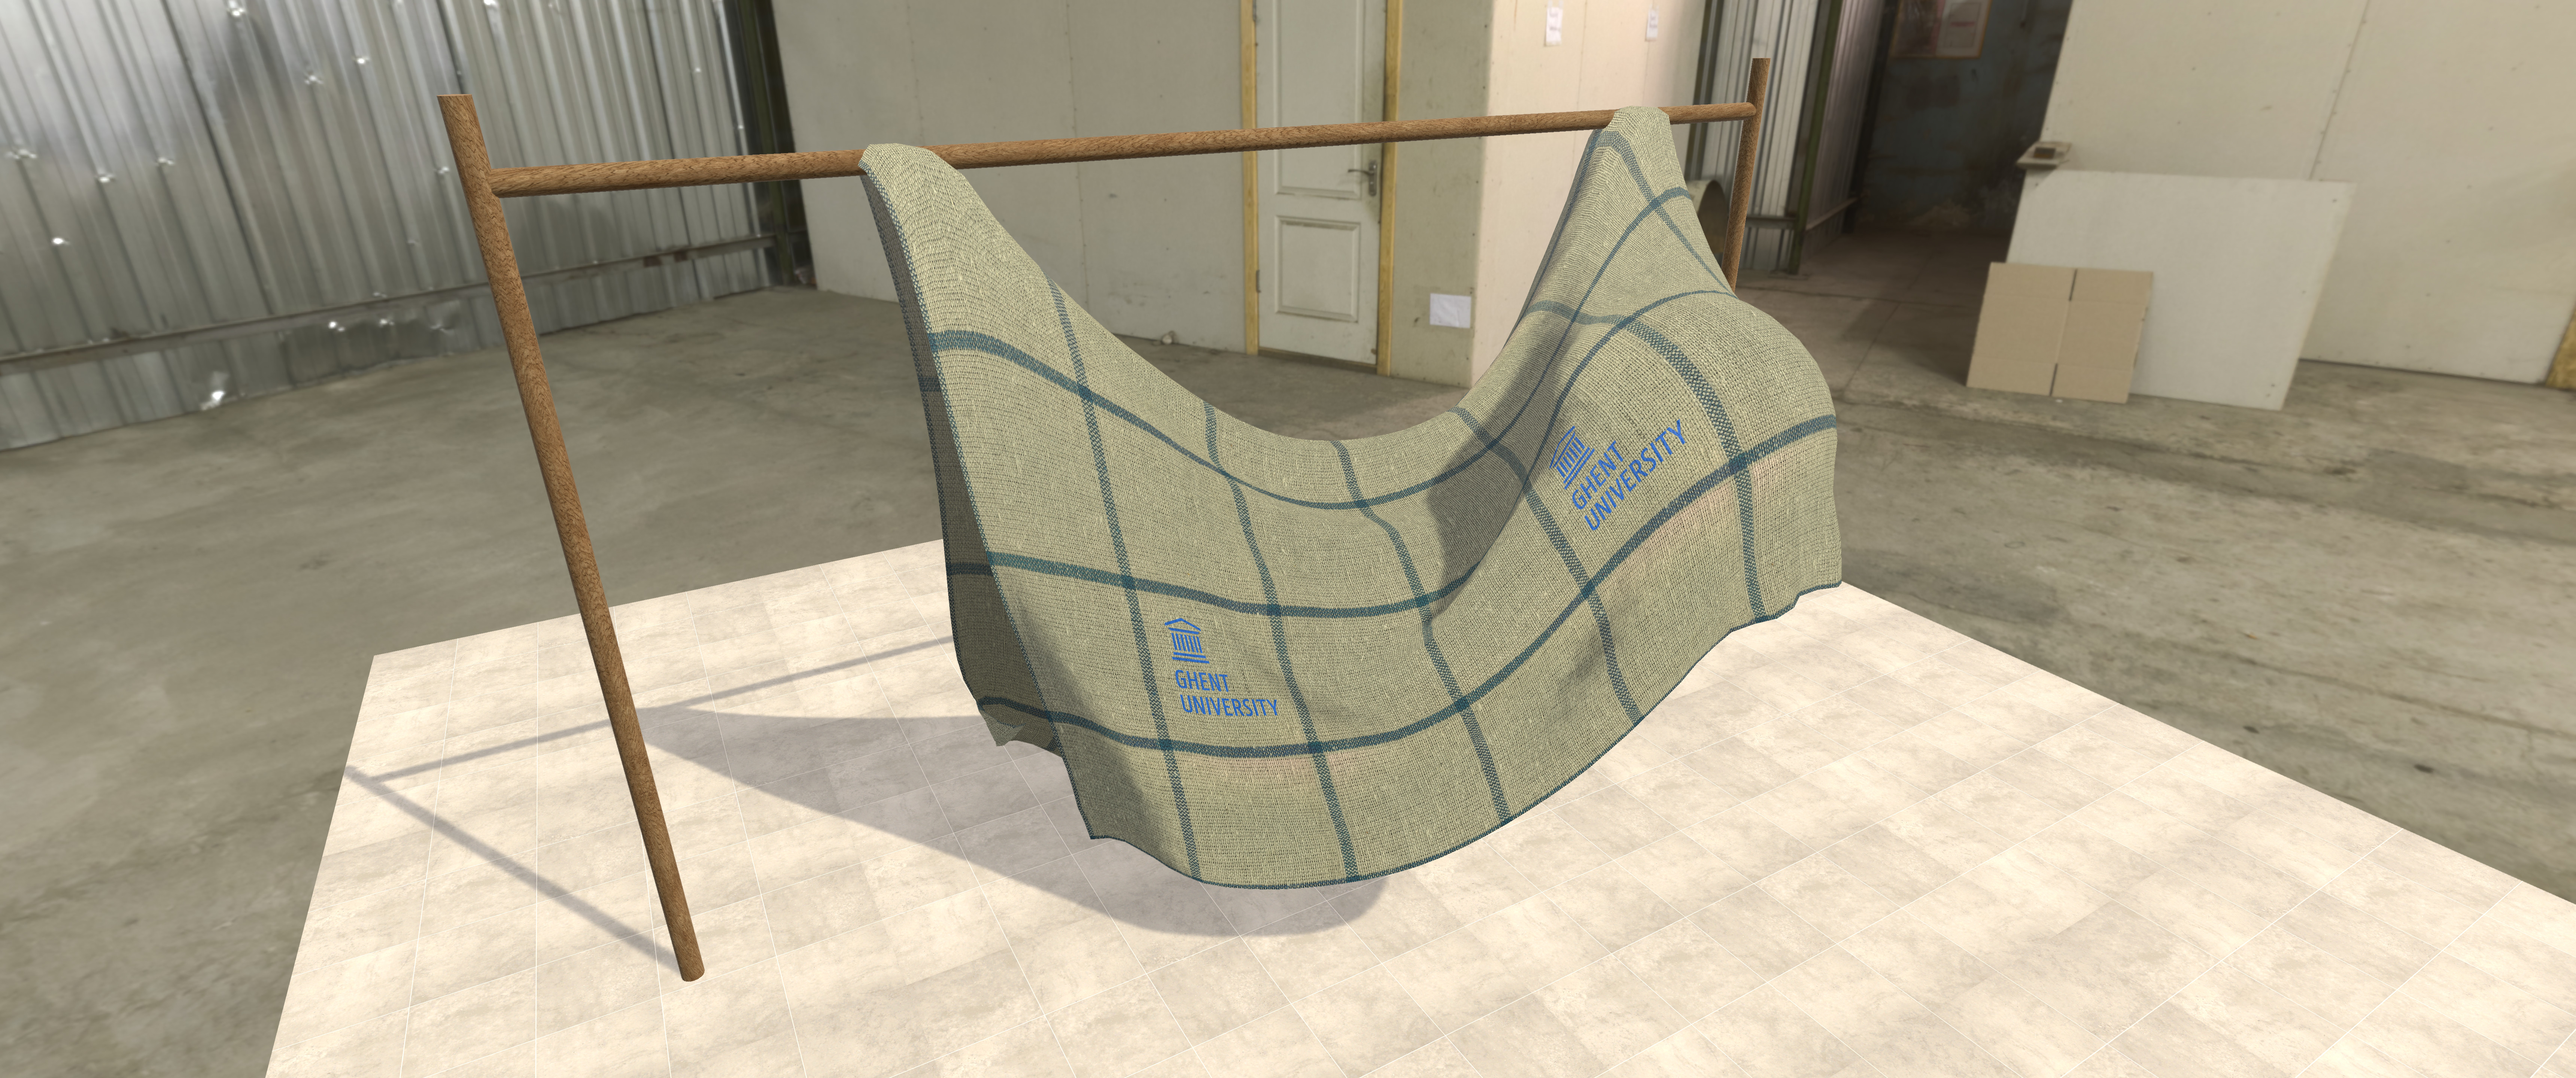
\includegraphics[width=\textwidth]{\home/chapters/04-simulation/figures/big_towel.jpg}
        \caption[Simulated, pinned rectangular cloth.]{A large rectangular cloth attached with two points to the bar. An invisible sphere on the right of the picture demonstrates sphere collisions.}
        \label{fig:towel_pinned}
    \end{subfigure}
    %\hfill
    \begin{subfigure}[b]{0.95\textwidth}
        \centering
        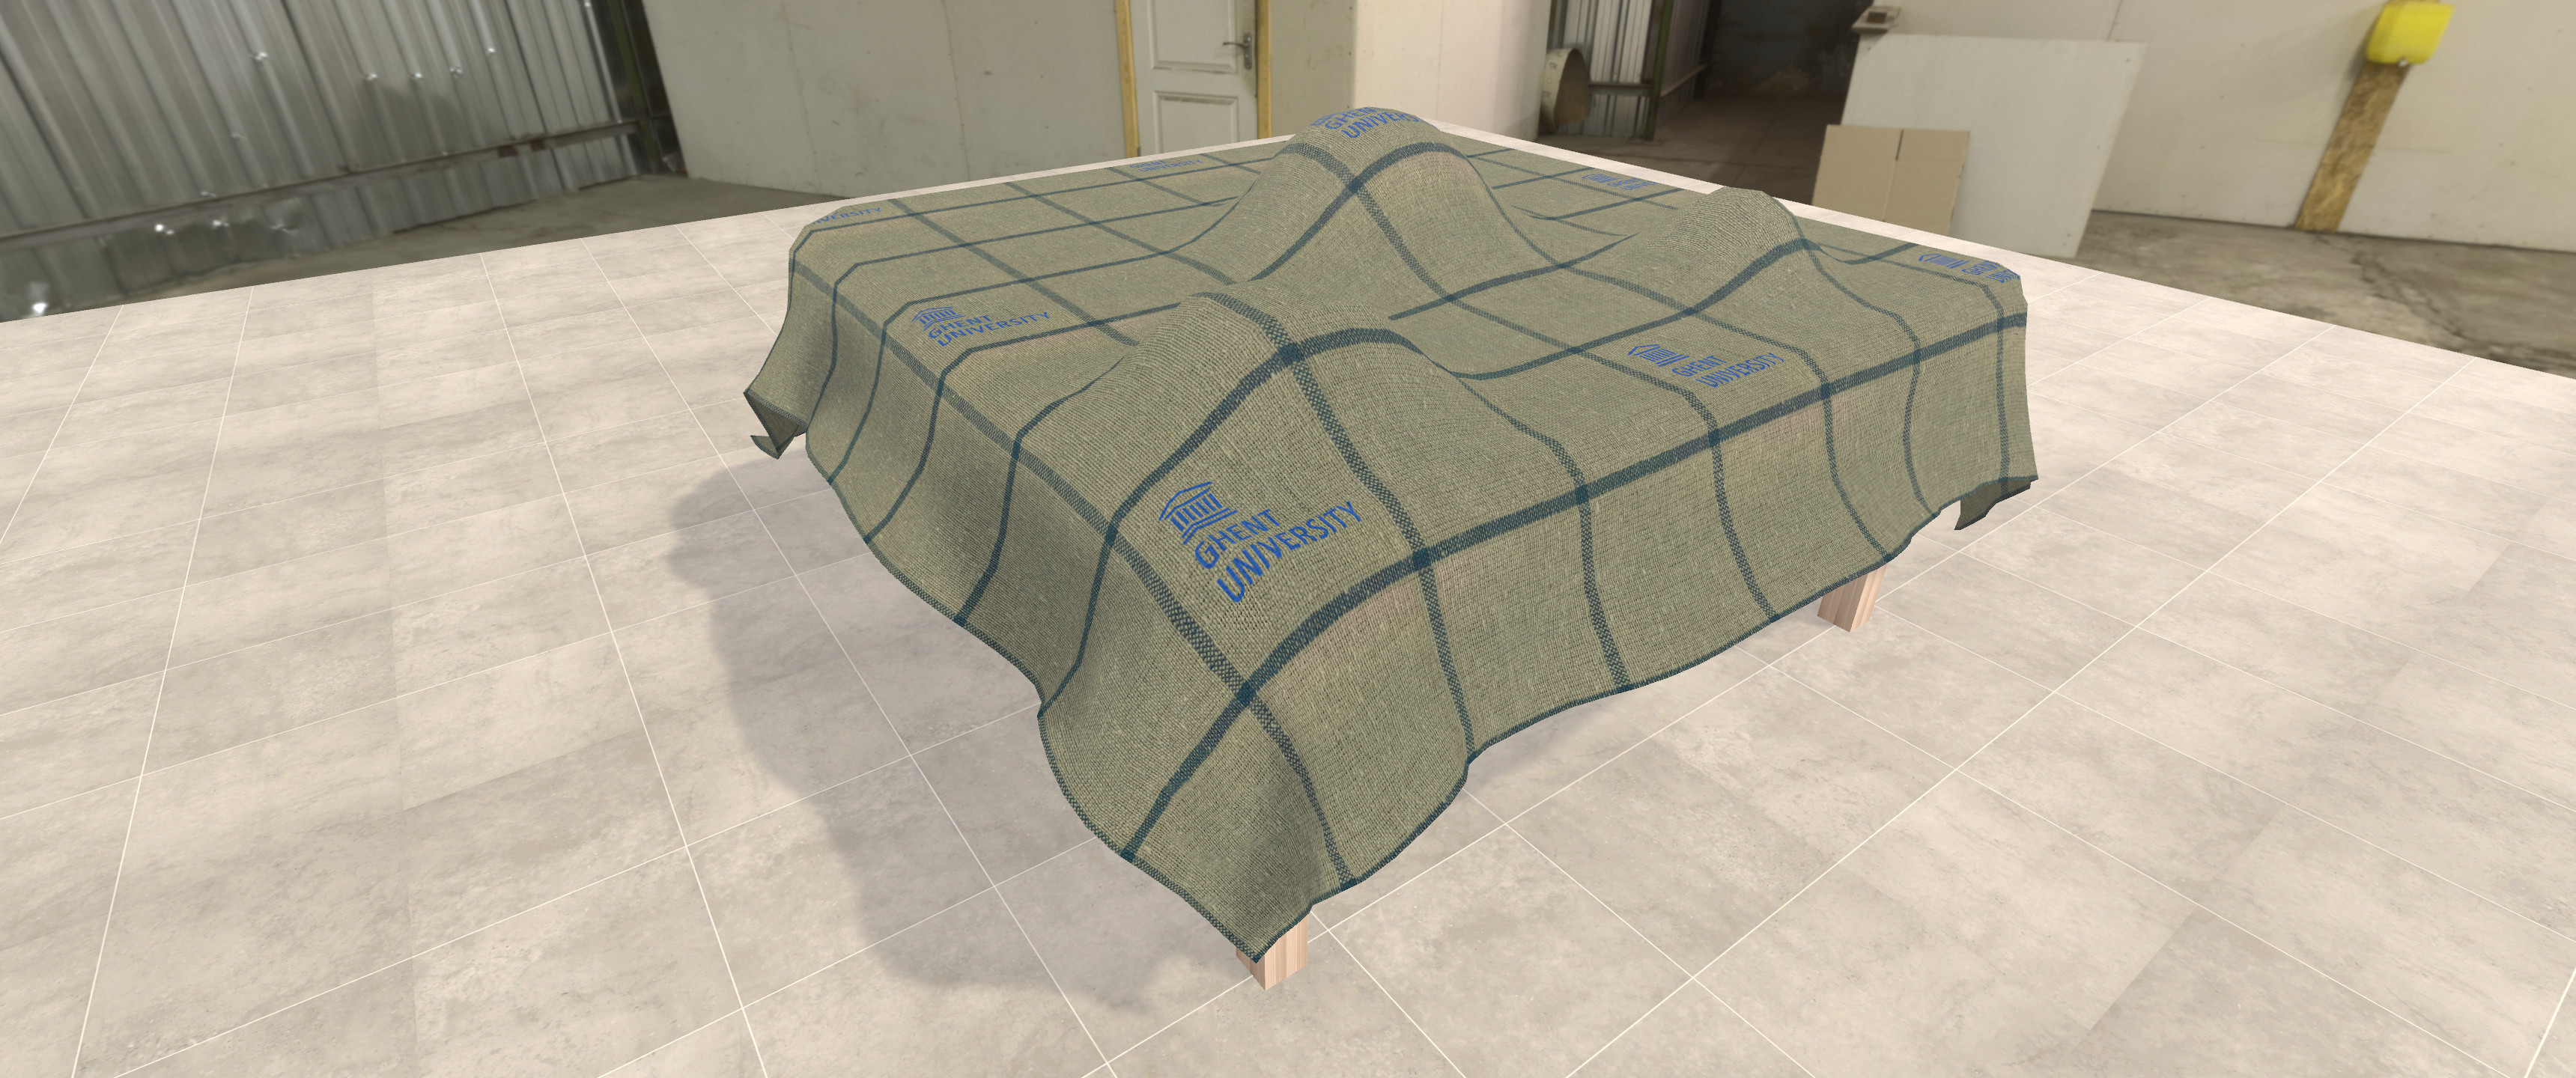
\includegraphics[width=\textwidth]{\home/chapters/04-simulation/figures/cloth_table.jpg}
        \caption[Simulated rectangular cloth on table.]{A large rectangular cloth draped on a table with spheres of different sizes.}
        \label{fig:towel_table}
    \end{subfigure}
    %\hfill
    \begin{subfigure}[b]{0.95\textwidth}
        \centering
        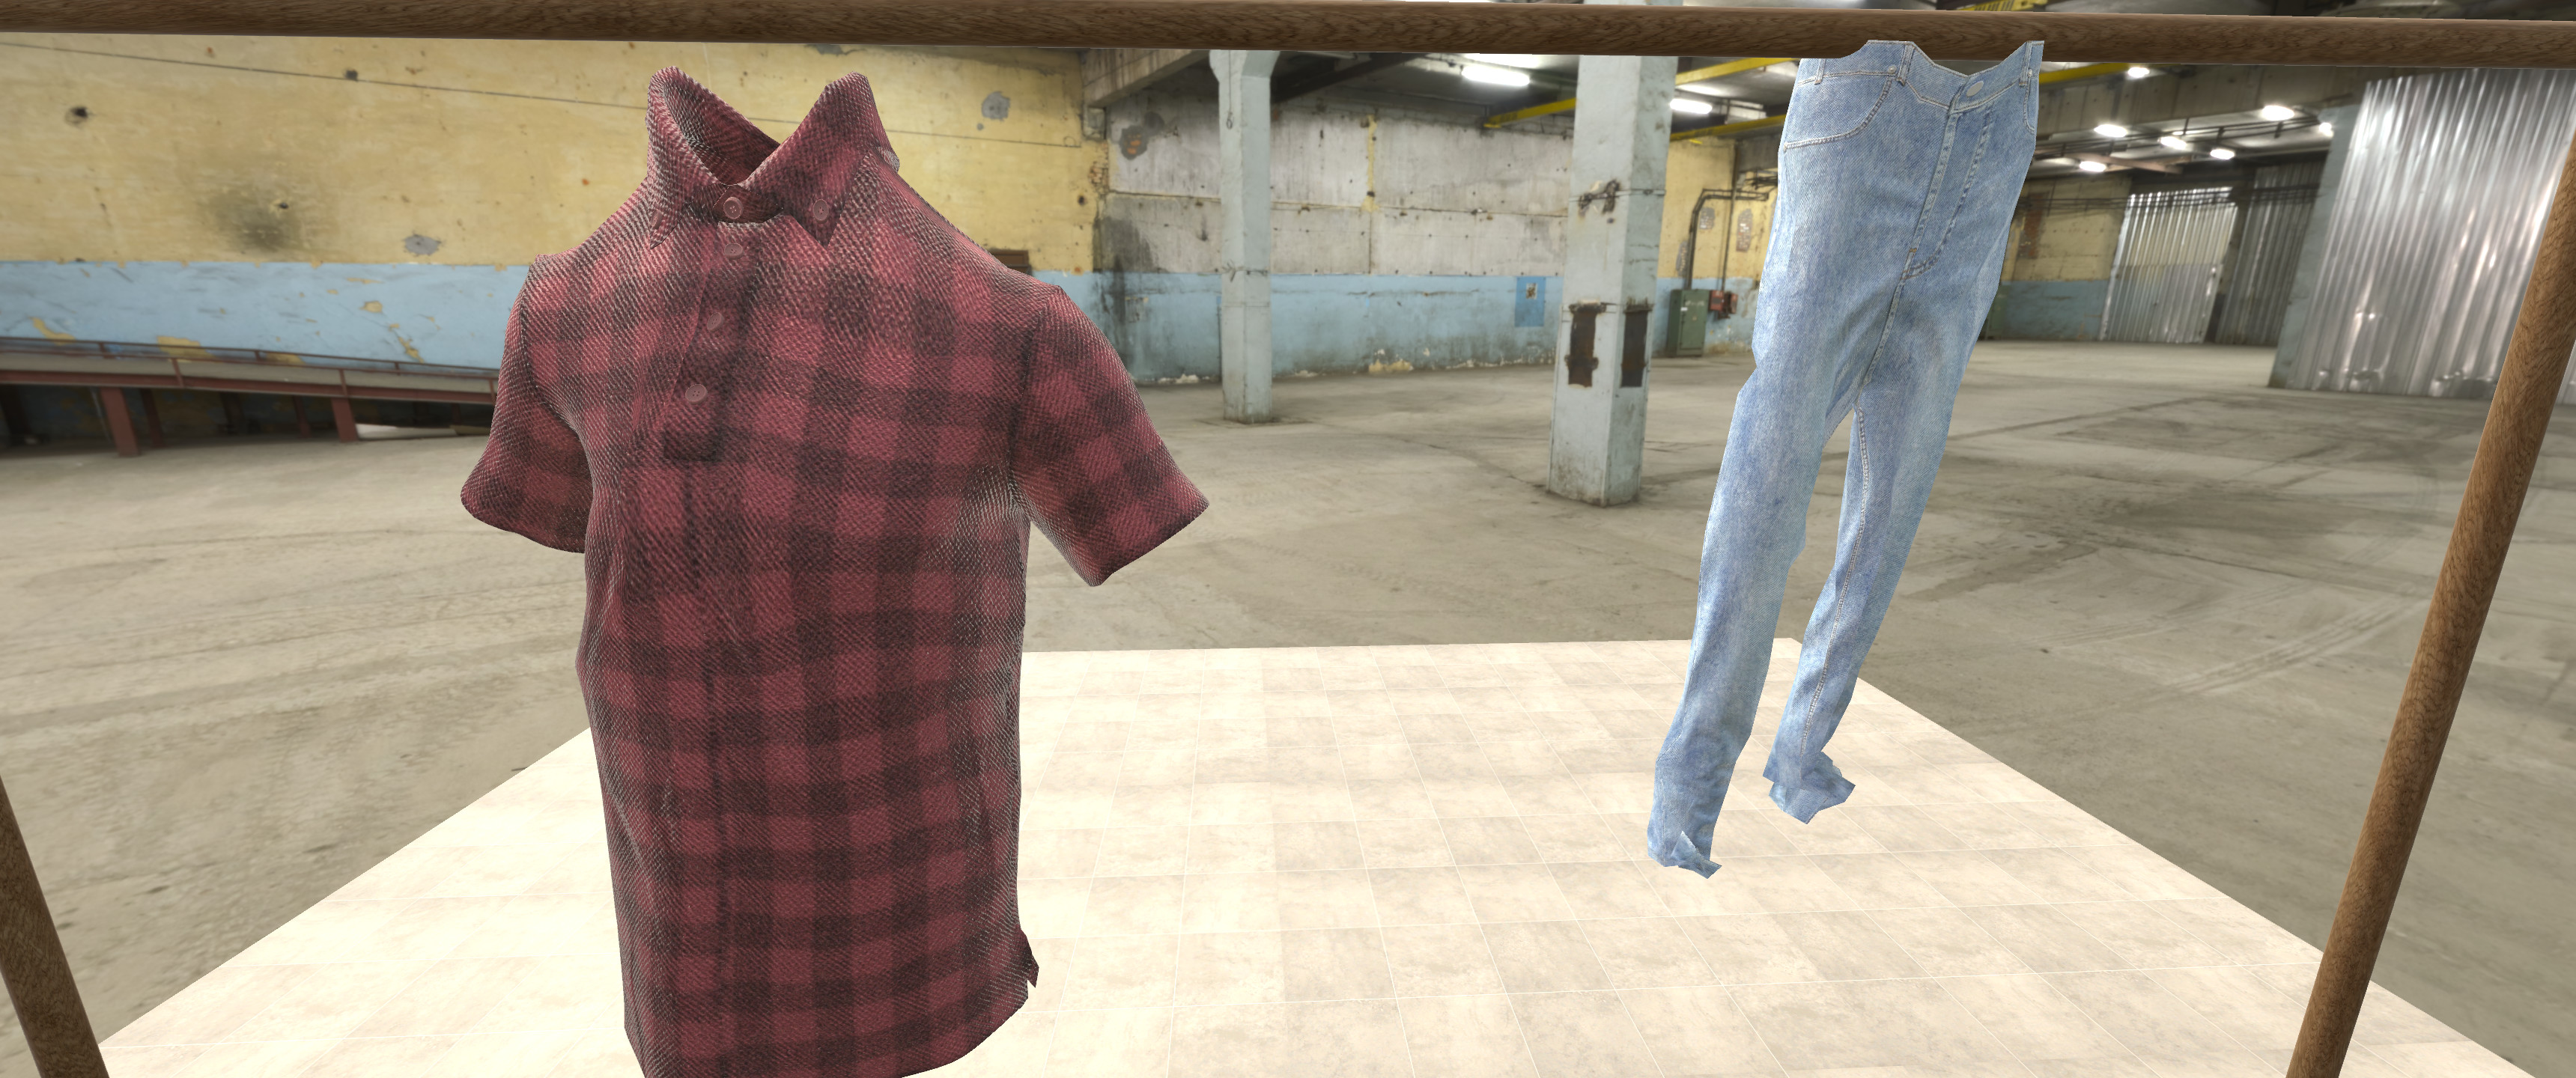
\includegraphics[width=\textwidth]{\home/chapters/04-simulation/figures/cloth_mesh.jpg}
        \caption[Simulated cloth meshes.]{A simulated shirt and trousers from arbitrary meshes.}
        \label{fig:cloth_sim_mesh}
    \end{subfigure}

    \caption[Spring-mass particle system for cloth demonstration.]{Spring-mass particle system for cloth demonstration.}
    \label{fig:cloth_sim_result}
\end{figure}

\section{Learning to fold in simulation}
% hier moet ik nog wat nadenken over het doel van deze sectie 
% het demonstreren dat de simulator werkt, dat plooien kan 
% tonen dat DRL werkt maar veel iteraties nodig heeft. De reward functie is godmode en moeilijk te transfereren naar het echt 
% eventueel een behavioural cloning approach ook tonen. Dan showcasen waar het zich vastrijdt
% eventueel iets over sim2real problemen dat hier al naar boven komen 
\subsection{Deep reinforcement learning setup for cloth folding in simulation}
In order to learn to fold cloth in simulation with a dual robotic arm, we use the \gls{DQN} algorithm with small stabilization and accelerations improvements. We first describe DQN, followed by our task setup.

\subsubsection{Deep Q-learning algorithm}

\Gls{DQN} is a variant of the Q-learning algorithm \autocite{watkins1992q} using deep neural networks using a replay buffer and stabilization tricks, as described in \cref{subsec:lit_rl}. On top of the two stabilization improvements, we implement two additional ways to accelerate learning: prioritized replay and double DQN.
Prioritized replay \autocite{schaul2015prioritized} recognizes that not all observations in the replay buffer are equally important. By sampling the replay buffer proportional to the TD-error (see \cref{eq:q-learning-update-rule}), experiences in which the agent made large prediction errors are more sampled. Prioritized sampling introduces bias that can be solved by annealed importance sampling.
Double DQN \autocite{van2016deep} addresses overestimation bias caused by the $\argmax$ operator in the \gls{DQN} update rule \cref{eq:q-learning-update-rule}. This is done by selecting the next best action using the online network while use the target network for getting the corresponding Q-value.
The full pseudocode is given in \cref{pseudocode:dqn}.

\begin{algorithm}[htpb]
    \DontPrintSemicolon

    \SetKwInOut{KwIn}{Input}

    \KwIn{Discount factor $\gamma$, minibatch size $k$, target network update frequency $C$, prioritization factor $\alpha$ and importance sampling exponent $\beta$, learning rate $\eta$}

    Initialize prioritized replay memory $\mathcal{H}=\varnothing$, $\Delta = 0$, $p_1=1$\;
    Initialize online action-value function $Q_{\theta}$ with random weights $\theta$\;
    Initialize target action-action function $Q_{\theta^{\prime}}$ with weights $\theta^{\prime}$\;

    \ForEach{episode}{

    Observe $s_0$\;

    \ForEach{step of episode}{
    Sample action $a_t \sim\ \pi_\theta(s_t)$\;
    Execute action $a_t$\;
    Observe reward $r_t$, new state $s_{t+1}$\;
    Store transition $\tuple{s_t, a_t, r_t, s_{t+1}}$ in $\mathcal{H}$ with maximal priority $p_t = \max_{i<t} p_i$\;

    \For{ $j=1$ \KwTo $k$}{
    Sample transition $j \sim P(j)=p_{j}^{\alpha} / \sum_{i} p_{i}^{\alpha}$\;
    Compute importance-sampling weight $w_{j}=(N \cdot P(j))^{-\beta} / \max _{i} w_{i}$\;
    Compute TD-error $\delta_{j}=r_{j}+\gamma Q_{\theta^{\prime}}\left(s_{j}, \argmax_{a} Q_{\theta}\left(s_{j}, a\right)\right)-Q_{\theta}\left(s_{j-1}, a_{j-1}\right)$\;
    Update transition priority $p_{j} \leftarrow\left|\delta_{j}\right|$\;
    Accumulate weight-change $\Delta \leftarrow \Delta+w_{j} \cdot \delta_{j} \cdot \nabla_{\theta} Q_{\theta}\left(s_{j-1}, a_{j-1}\right)$\;
    }

    Update weights $\theta \leftarrow \theta+\eta \cdot \Delta$\;
    Reset gradients $\Delta = 0$\;
    Every $C$ steps: update target network $\theta^{\prime} \leftarrow \theta$\;
    }
    }
    \caption{Double \gls{DQN} with prioritized experience replay}
    \label{pseudocode:dqn}
\end{algorithm}


\subsubsection{Task description}
We define the task as performing a double fold in a rectangular piece of cloth by using a task structure. The tasks consist of grasping the corners of the cloth, then folding it inwards and releasing it. Afterwards, a second fold is executed by regrasping the corners and performing the final fold.
The state space $\mathcal{S} \in \mathbb{R}^{114}$ consists of the joint angles of the Baxter robot and the positions of the cloth particles relative to the robot end-effectors.
The action space $\mathcal{A} \in \mathbb{R}^{42}$ is in joint space: for every joint, the agent can move according to a fixed angle in any direction.
We provide a distance-based reward function $R$ which incorporates the distance between the corner points their current location and target location. Additionally, we include auxiliary objectives to provide a more rich reward signal to the agent: maximize the stretch of the cloth in order to minimize wrinkles.
\begin{align} \label{eq:sim_cost_function}
    \operatorname{Cost} = & w_1 \sum_{p \in \cloth_f} \operatorname{dist}{\left( \vec{x}_p , \vec{x}_{p}^{*} \right)} + \nonumber                                            \\
                          & w_2 \sum_{p \in \cloth_f} \operatorname{dist}{\left( \vec{x}_{\text{ee}} , \vec{x}_{p} \right)} + \nonumber                                      \\
                          & w_3 \sum_{p \in \cloth_b} \sum_{p^{\prime} \in \cloth_b, p^{\prime} \neq p} \operatorname{dist}{\left( \vec{x}_p , \vec{x}_{p^{\prime}} \right)}
\end{align}
The coefficients $w_1,w_2, w_3$ are weights for trading-off the reward function components. The particles in $\cloth_f$ are the particles for which we manually specified a target location in order to fold. $\vec{x}_{p}^{*}$ is the target location of the particle and $\vec{x}_{\text{ee}}$ is the current position of the end-effector. $\cloth_b$ are the particles lying at the boundary of the cloth. We aim to maximize the distance between the boundary nodes in order to minimize wrinkles.
We multiply the cost function $\operatorname{Cost}$ with minus one for passing a reward for the agent.
In our experiments, we represent the Q-function with a feedforward neural network containing two layers with 128~\texttimes~64 hidden neurons.


\subsection{Results}
When training the agent to learn how to fold a cloth twice, we notice a significant difference in learning speed between the different stages of the task. We are able to quickly learn how to grasp the cloth when it is in two unfolded configurations. In \cref{sub@fig:sim_results_grasp_1}, the cloth initial layout is completely unfolded and the agent progressively learns to grasp the cloth. In the succeeding grasping task in \cref{sub@fig:sim_results_grasp_2}, the cloth is already folded once. In this scenario, we see the agent learning the task at a similar pace to the first grasp. On the other hand, learning to fold when grasping the cloth is more difficult and requires roughly 31 times more interactions with environment as visible in \cref{sub@fig:sim_results_fold_1} and \cref{sub@fig:sim_results_fold_2}. The main reason for the folding task requiring more interactions compared to grasping can be found by considering the dynamics complexity of both tasks. The grasping tasks are essentially reaching tasks in which the agent must find the optimal path from the starting pose of the end-effector to the target particles. Once the agent finds the target locations, the particles are snapped to the end-effector due to undermodelling the contact dynamics. In contrast, during folding, the agent must find a trajectory that achieves the fold without causing wrinkles or sliding the cloth from the table. Small perturbations and random action exploration then leads to large changes in the received reward which renders the optimization landscape more difficult. Nevertheless, we find that the agent is able to learn the task within \qty{24}{\hour} of training time.
The success rates and training times we find are comparable to similar experiments in other work \autocite{Matas2018,jangir2020dynamic}. However, exact comparisons and benchmarking is difficult due to each work using different robotics simulators, cloth physics simulation models and learning algorithms.
% onze simulatie voelt ook meer aan als wavy water. er zit meer energie in wat vouwen moeilijker maakt

In \cref{fig:sim_results_success_rate_test}, we evaluate the success rate per stage in the task. We run this evaluation by letting the agent sequentially execute the task: grasping the corners, performing a first fold, regrasping the corners that are now at a different position and performing the second fold. This task is performed 100 times with different starting locations of the robot grippers. We find that the robot successfully executes this task with \qty{97}{\percent} up to performing the second fold. During the last stage, the success rate drops due to the second folding operation failing \qty{26}{\percent} of the time. We hypothesize this is due to the cloth being in a more difficult configuration containing more energy caused by the first fold. In addition, slightly hitting the cloth can cancel the resulting first fold whereas hitting the cloth in the first fold causes some local wrinkles. Finally, the first fold is easier due to resetting the cloth repeatedly to the same starting configuration. Contrarily, the second fold starts from the result of the first fold which contains more variability. We show visualizations of the learned grasping and folding behaviour in \cref{fig:sim_drl_demo}.

\begin{figure}[p]{}
    \centering
    \begin{subfigure}[c]{0.49\textwidth}
        \centering
        \includegraphics[width=\textwidth]{\home/chapters/04-simulation/figures/Grasp_1_Reward_per_episode}
        \caption{Reward per episode for executing the first grasp.}
        \label{fig:sim_results_grasp_1}
    \end{subfigure}
    \hfill
    \begin{subfigure}[c]{0.49\textwidth}
        \centering
        \includegraphics[width=\textwidth]{\home/chapters/04-simulation/figures/Fold_1_Reward_per_episode}
        \caption{Reward per episode for executing the first fold.}
        \label{fig:sim_results_fold_1}
    \end{subfigure}

    \vskip\baselineskip

    \begin{subfigure}[c]{0.49\textwidth}
        \centering
        \includegraphics[width=\textwidth]{\home/chapters/04-simulation/figures/Grasp_2_Reward_per_episode}
        \caption{Reward per episode for executing the second grasp.}
        \label{fig:sim_results_grasp_2}
    \end{subfigure}
    \hfill
    \begin{subfigure}[c]{0.49\textwidth}
        \centering
        \includegraphics[width=\textwidth]{\home/chapters/04-simulation/figures/Fold_2_Reward_per_episode}
        \caption{Reward per episode for executing the second fold.}
        \label{fig:sim_results_fold_2}
    \end{subfigure}

    \caption[Mean reward per episode for the subtasks during training.]{Mean reward per episode for the subtasks of learning how to fold a cloth twice in simulation. Each plot represents the progress for a certain subtask.}
    \label{fig:sim_results_reward}
\end{figure}

% \begin{figure}[htbp]
%     \centering
%     \includesvg[width=\textwidth]{figures/reward_per_episode.svg}
%     \caption[Mean reward per episode for the subtasks during training.]{Mean reward per episode for the subtasks during training.}
%     \label{fig:sim_results_reward}
% \end{figure}

\begin{figure}[htbp]
    \centering
    \includegraphics[width=\textwidth]{\home/chapters/04-simulation/figures/total_success_rate}
    \caption[Success rate at test time for folding cloth twice in simulation.]{Success rate per subtask at test time for folding cloth twice in simulation.
    }
    \label{fig:sim_results_success_rate_test}
\end{figure}

\begin{figure}[htpb]{}
    \centering
    \begin{subfigure}[b]{\textwidth}
        \centering
        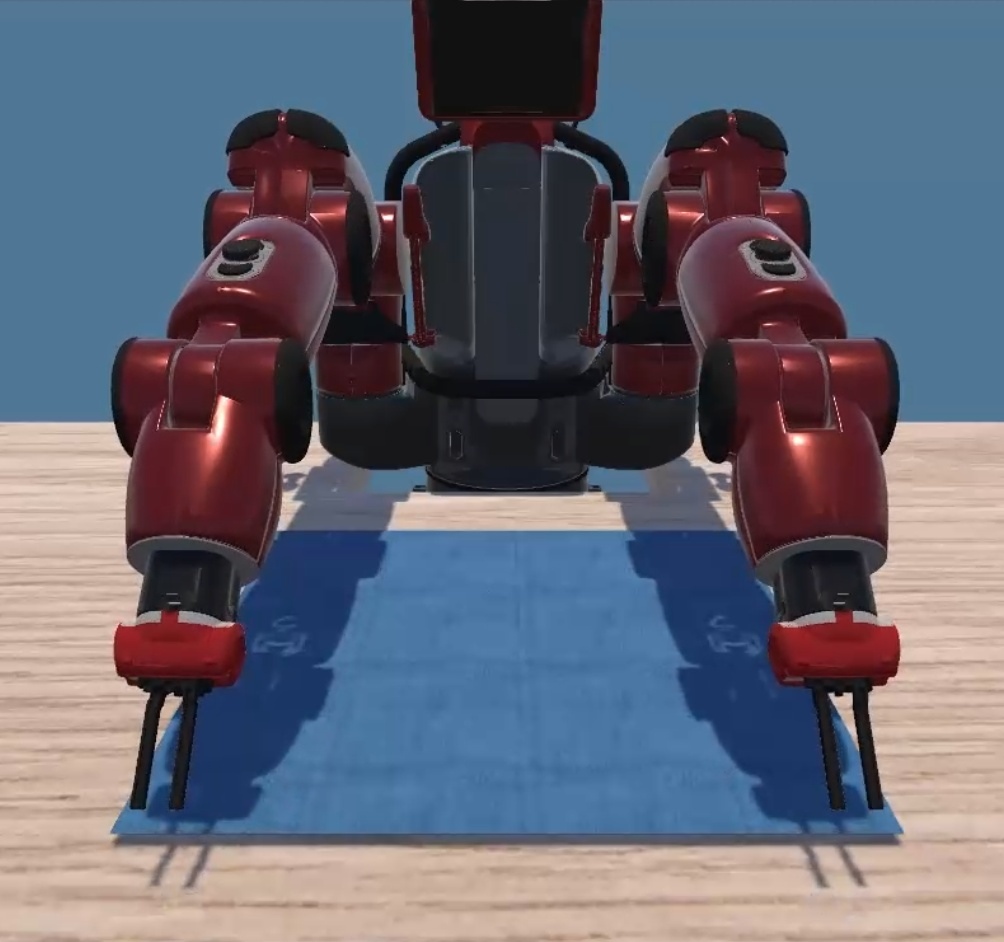
\includegraphics[width=0.5\textwidth,height=0.30\textheight]{\home/chapters/04-simulation/figures/baxter_grasp1.jpg}
        \caption{Baxter reaching towards cloth corner points.}
        \label{fig:baxter_results_grasp1}
    \end{subfigure}

    \begin{subfigure}[b]{\textwidth}
        \centering
        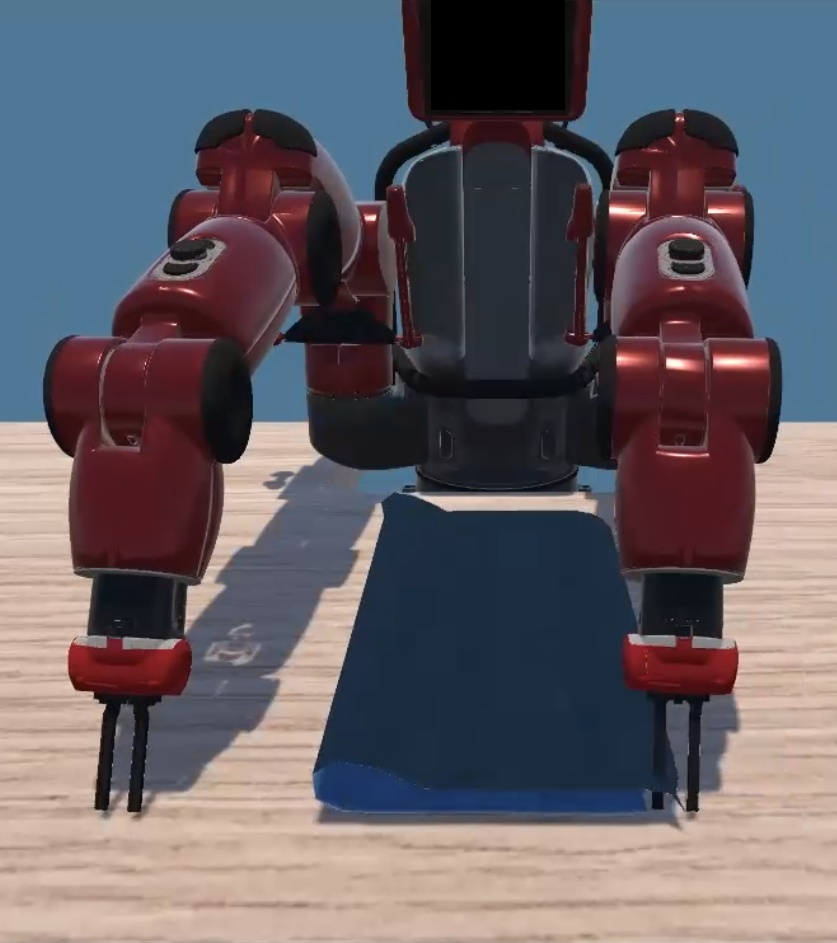
\includegraphics[width=0.5\textwidth,height=0.30\textheight]{\home/chapters/04-simulation/figures/baxter_fold1.jpg}
        \caption{Baxter successfully performing the first fold.}
        \label{fig:baxter_results_fold1}
    \end{subfigure}

    \begin{subfigure}[b]{\textwidth}
        \centering
        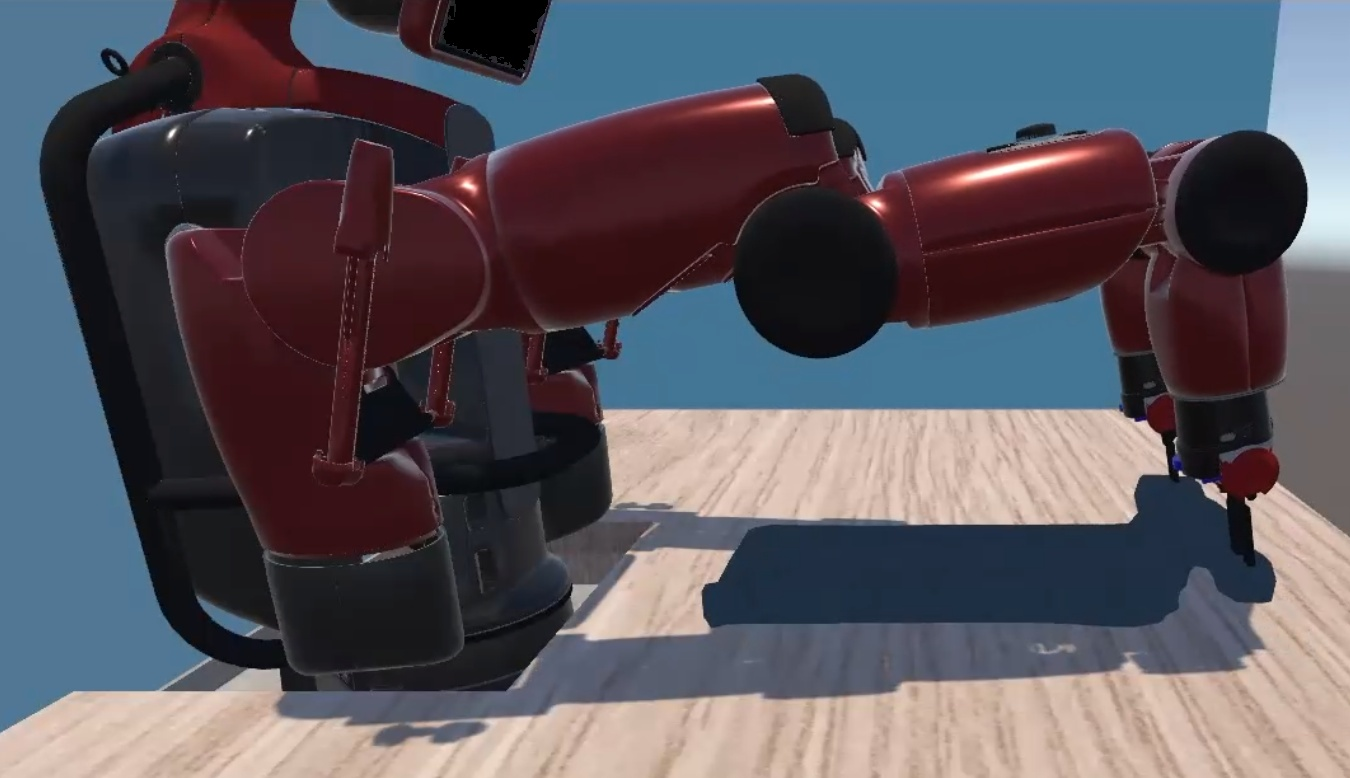
\includegraphics[keepaspectratio,height=0.20\textheight]{\home/chapters/04-simulation/figures/baxter_fold2.jpg}
        \caption{Baxter performing the second fold.}
        \label{fig:baxter_results_fold2}
    \end{subfigure}

    \caption[]{Visualizations of the learned grasping and folding behaviour.}
    \label{fig:sim_drl_demo}
\end{figure}

\section{Conclusion}
Simulation is an indispensable tool for the robotics researcher as it allows fast experimentation and massive, inexpensive data generation. The robotics simulator landscape is large, and choosing a specific technology requires specifying and trading-off domain-specific requirements. For our application of cloth folding, we found the support for cloth simulation in existing robotics simulators to be lacking. Therefore, we decided to use Unity as robotics simulator and implement a custom cloth simulation on GPU using a mass-spring methodology. We found that a \gls{DQN} agent can learn to fold a rectangular piece of cloth twice in simulation within \qty{24}{\hour} of wall time on standard computational hardware. However, it is unclear whether such an approach transfers to the real world.
First, Sim2Real methods like domain randomization can be used for transfer but require a lot of computational power.
Second, we require a lot of interactions in simulation. Learning from scratch on a real robot would take an exorbitant amount of time. Assuming a roll-out would consume one minute of robot time, this experiment would almost last half a year to complete.
Third, the cloth state is used both as input observation for the agent and calculating the reward function. However, obtaining the state of the cloth in the real world is non-trivial.
In the next chapter, we will provide a solution for these issues: estimating the cloth state using sensors and learning directly on the physical platform.

\end{document}